
\documentclass{frontiersSCNS} % for Science articles

\usepackage{url,lineno}
%\linenumbers

%----------------------------------------------------------------------
% Own stuff
\usepackage{ucs}
\usepackage[utf8x]{inputenc}
\newcommand{\tbw}[1]{{\bf\parindent0pt\color{red}#1}}
\usepackage{minted}
\newminted{python}{showspaces=false,
  showtabs=false,
%  linenos=true,
  fontsize=\tiny,
  mathescape=true,
  frame=leftline,
  framerule=0pt,
  framesep=0mm}
%----------------------------------------------------------------------

\copyrightyear{}
\pubyear{}

\def\journal{Neuroinformatics}%%% write here for which journal %%%
\def\DOI{}
\def\articleType{Research Article}
\def\keyFont{\fontsize{8}{11}\helveticabold }
\def\firstAuthorLast{Djurfeldt {et~al.}}
\def\Authors{Mikael Djurfeldt\,$^{1,2,*}$, Andrew P. Davison\,$^{3}$,
 Hans Ekkehard Plesser\,$^{4,5}$, and Jochen M. Eppler\,$^5$}
% Affiliations should be keyed to the author's name with superscript
% numbers and be listed as follows: Laboratory, Institute, Department,
% Organization, City, State abbreviation (USA, Canada, Australia), and
% Country (without detailed address information such as city zip codes
% or street names).  If one of the authors has a change of address,
% list the new address below the correspondence details using a
% superscript symbol and use the same symbol to indicate the author in
% the author list.
\def\Address{$^{1}$PDC Center for High-Performance Computing, KTH
  Royal Institute of Technology, Stockholm, Sweden\\
  $^{2}$International Neuroinformatics Coordinating Facility (INCF),
  Stockholm, Sweden\\
  $^{3}$Unité de Neurosciences, Information et Complexité (UNIC),
  CNRS, Gif sur Yvette, France\\
  $^{4}$Department of Mathematical Sciences and Technology, Norwegian
  University of Life Sciences, Aas, Norway\\
  $^{5}$Institute of Neuroscience and Medicine (INM-6) and Institute
  for Advanced Simulation (IAS-6), Jülich Research Centre and
  JARA, Jülich, Germany}
% The Corresponding Author should be marked with an asterisk Provide
% the exact contact address (this time including street name and city
% zip code) and email of the corresponding author
\def\corrAuthor{Mikael Djurfeldt} \def\corrAddress{International
  Neuroinformatics Coordinating Facility (INCF), Nobels väg 15 A,
  Stockholm, SE-17177, Sweden} \def\corrEmail{djurfeldt@incf.org}

% \color{FrontiersColor} Is the color used in the Journal name, in the
% title, and the names of the sections


\begin{document}
\onecolumn
\firstpage{1}

\title[CSA in NEST and PyNN]{Modeling connectivity: Connection-set
 Algebra in NEST and PyNN}
\author[\firstAuthorLast ]{\Authors}
\address{}
\correspondance{}
\extraAuth{}% If there are more than 1 additional author, comment this
%line and uncomment the next one
%\extraAuth{corresponding Author2 \\ Laboratory X2, Institute X2,
%Department X2, Organization X2, Street X2, City X2 , State XX2 (only
%USA, Canada and Australia), Zip Code2, X2 Country X2,
%email2@uni2.edu}
\topic{Python in Neuroscience 2}

\maketitle
\begin{abstract} % maximum 2000 characters including spaces

Most neuronal network simulators provide simulator-specific methods
for specifying connectivity. In addition, several universal
description languages for neuronal network models (e.g. PyNN, NeuroML
and NineML) have been developed. Usually, there is a choice between
explicitly specifying individual connections or selecting one of a
predefined set of connection primitives. Such primitives are well
suited for building random balanced networks, synfire chains and
recurrent networks without much structure. However, they often either
lack the required expressiveness or their implementations lack the
required computational efficiency to specify the connectivity of
complex hierarchical network models now under investigation.

The connection-set algebra \citep[CSA;][]{djurfeldt12} is a formalism
for specifying the connectivity of neuronal network models. CSA
provides operators to combine simpler connectivities into more complex
ones and also provides parameterization of such sets. The CSA is
expressive enough to describe a wide range of connectivities and can
serve as a concise notation for network structure in scientific
writing as well as in model description code for neural
simulations. CSA implementations allow for scalable and efficient
representation of connectivity in parallel neuronal network
simulators.

Here, we describe the use of CSA and how it is coupled to the neural
simulation tool NEST \citep{Gewaltig_07_11204} through the new
ConnectionGenerator interface provided by the libneurosim library. We
demonstrate how CSA can be used for the specification of connectivity
in simulator-independent neural specification language PyNN
\citep{Davison09} and how using CSA, as a high-level representation of
connectivity patterns, avoids performance penalties and results in
good scalability when transferred to the simulator.

\tiny
 \keyFont{ \section{Keywords:} model description, connectivity,
 neural simulation, Python, large-scale modeling } %All article
 %types: you may provide up to 8 keywords; at least 5 are mandatory.
\end{abstract}

\section{Introduction}

Currently, most simulators use their own methods for describing
connections between neurons. This makes it hard for users to port
models from one simulator to another and leaves the efficient
implementation of connection-generating functions as a task to the
simulator developers. Especially in a parallel environment, this is
not a trivial pursuit. One way to ease this problem is the use of
general connection-generating libraries like the Connection-set
Algebra \citep[CSA;][]{djurfeldt12} or the graph library developed for
NineML \citep{raikov10}. They allow a simulator-independent
specification of connectivity and comprise a compact description of
connectivity, which can be efficiently transferred between different
levels of simulation description languages.

To take account of the fact that different users prefer different
simulators and also might prefer different libraries to create
connectivity, we created a generic \emph{Connection Generator}
interface. It enables the use of CSA and similar libraries in
different neuronal simulators. The interface makes both the simulator
and the connection-generating library replaceable and therefore gives
maximum flexibility to the user.

The remainder of this section will introduce related work and the
different components (CSA, PyNN, NEST) that were made to work with the
Connection Generator interface. The remaining sections will explain
the interface itself and our modifications and extensions to the
components and the interplay between them. We provide benchmark
results that demonstrate the excellent scaling of the implementation
of the interface and close with a discussion of the interface and an
outlook to further extensions.

%----------------------------------------------------------------------

\subsection{NineML}
\tbw{To be written}
\subsection{NeuroML}
\tbw{To be written}
\subsection{CSA}
\tbw{To be written}

%----------------------------------------------------------------------

\subsection{PyNN}

PyNN \citep[http://www.neuralensemble.org/PyNN;][]{Davison09} is a
community effort to provide a simulator-independent API to describe
neuronal networks in Python. In PyNN, the network is built from
Populations of neurons and Projections between them. Each Projection
is created by a Connector, which knows how to set up the single
connections. Different Connectors exist and allow to set up a variety
of different connection patterns.

However, one of the regular problems with this approach is, that PyNN
needs to break up the compact description of connectivity given by
users into the commands understood by the respective backend. These
are often already too low-level (e.g. convergent or divergent
connects, one-to-one connects) and thus entail a certain performance
penalty due to data transfer and function call overhead. This is
especially problematic when randomly parametrized parameters are used
(and drawn in Python), because this makes one-to-one connects the only
possibility for transferring the connection information into the
simulator.

The problem of excessive data transfers between PyNN and the simulator
can be solved by passing a compact description of (possibly random)
connectivity to the simulator. This representation can then be
iterated and expanded only on the simulator level and thus avoid
overhead. Moreover, this also allows the efficient parallelization on
the lower software layers.

Since version 0.7, PyNN provides the CSAConnector, which can iterate a
CSA connection set and issue one-to-one connect calls at the different
backends. During this study, we extended PyNN with a new and
specialized CSAConnector, which passes the complete CSA object down to
the simulator to reduce the overhead. The details of this effienct
interface are described in Section \ref{sec:conn_gen_pynn}. Section
\ref{sec:benchmarks} contains benchmarking results of the different
implementations of the CSAConnector and the native NEST connection
routines.

\subsection{NEST}

NEST is a simulator for large networks of point neurons or neuron
models with few electrical compartments
\citep[http://www.nest-initiative.org;][]{Gewaltig_07_11204}. It is
suited for a broad range of neuronal network modeling approaches and
runs on a large variety of computer architectures. NEST is
parallelized using OpenMP \citep{OpenMPSpec} and MPI
\citep{MPIForum94} and scales well on large clusters of multi-core
processors and supercomputers \citep{Helias12_26}.

The network description is a script, written either in SLI, NEST's
built-in simulation language, or in Python, using the Python interface
to NEST \citep[PyNEST;][]{Eppler09_12}. The following description uses
the PyNEST syntax if not noted otherwise. To build a network in NEST,
the user first creates the neurons of the network and devices for
stimulation and measurement using the \texttt{Create()} function and
then connects the elements with each other. NEST provides two basic
ways for creating connectivity.

\subsubsection*{Native connection functions:}

The most basic connect function, \texttt{Connect()}, takes a list of
pre-synaptic neurons (or devices) and a list of the same amount of
post-synaptic neurons (or devices) and connects them in a one-to-one
fashion. Because of the function call overhead, this function is not
very efficient to connect up large networks.

For such cases, the connection functions \texttt{ConvergentConnect()}
and \texttt{DivergentConnect()} can be used to create multiple
connections with a single call. In addition, random variants for both
functions exist to support the user in creating networks on the basis
of statistic knowledge. However, random parameters (e.g. weight,
delay) for the connections need to be drawn manually by the user and
supplied to NEST after the creation of connections.

\tbw{Should we add a figure here? Maybe the ones
  from\\ http://nest-initiative.org/index.php/Connection\_Management?}

\subsubsection*{Topology module:}

To ease the creation of networks with topological relations between
the neurons and organizations of neurons into layers and areas, NEST
provides a Topology module \citep{Plesser_13}. It supports the user in
connecting neurons and randomly initialize synapse parameters based on
toplogical measures in the network.

\tbw{Should we add a code listing or some more information on how to
  use the Toplogy module?}

A comparison of the performance of the Topology module to the native
connection routines and to the novel CSA interface to NEST is given in
Section \ref{sec:benchmarks}. The implementation of the Connection
Generator interface for NEST is explained in Section
\ref{sec:conn_gen_nest}.

%----------------------------------------------------------------------

\section{The Connection-set Algebra}\label{sec:csa}

The connection-set algebra \citep[CSA;][]{djurfeldt12} is a formalism
for network connectivity which can be used both when describing a
network to a fellow researcher and when implementing a model for a
simulator.  It is currently focused on connectivity which has a
constructive or statistical element, but it can also be used when all
network connections are given, or in cases where only elements of the
connectivity is pre-specified.

Some of the distinguishing aspects of CSA are:
\begin{itemize}
\item It is abstract. CSA deals with sets of \emph{connections}. A
  connection is basically just an edge in a graph, with associated
  parameters. There is a clean separation between CSA and other
  aspects of model or simulator infrastructure.
\item A connection-set can represent a \emph{type} of
  connectivity---a connectivity pattern---in addition to the connectivity
  of a specific network.
\item It is that it is an algebra: There are pre-existing
  connection-sets and operators to define new connection-sets in terms
  of existing.
\item It enables a succinct and precise description and definition of
  connectivity in terms of such algebraic expressions.
\item There are ways to implement CSA on a computer which are both
  efficient and scalable on a parallel computer.
\end{itemize}

%\subsection{Basic concepts}
%  \textbf{Figure 1.}{CSA Connection Matrix.}\label{fig:01}
%\subsection{Examples}
%  \textbf{Figure 2.}{An example of using CSA.}\label{fig:02}
%\subsection{Parallelization}
%\subsection{Implementation}
%\subsubsection{Masks}
%\subsection{Python wrapper}
%\subsection{Serialization/deserialization}
\tbw{To be continued...}

%----------------------------------------------------------------------

\section{The Connection Generator API}

To allow users to flexibly chose between simulators and the library,
which generates connectivity, we developed an interface (the
\emph{Connection Generator}) that abstracts the simulator and the
connection generating library from each other, making both the
simulator and the connectivity description library replaceable.

\begin{figure}[ht]
\centering
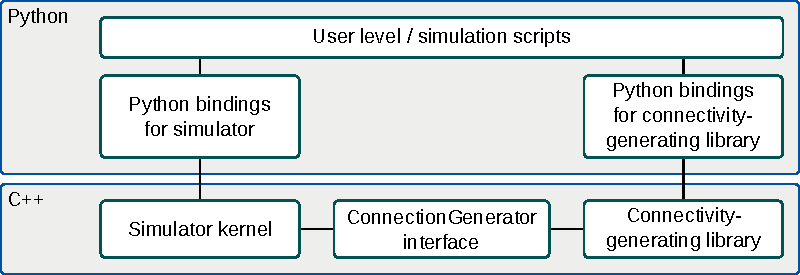
\includegraphics[scale=.8]{figures/block_diagram_conngen.pdf}
\caption{Block diagram of the Connection Generator interface and the
  components involved. The central component is the
  ConnectionGenerator class itself. It can connect to different simulators
  (e.g. NEST) and to different connection generating libraries
  (e.g. CSA). The user can use Python for all simulation
  tasks.}\label{fig:block_diagram_conngen}
\end{figure}

\tbw{To be written}

\subsection{The interface}

The interface is designed as an abstract base class in C++ and
consists of the following functions:

\begin{unlist}
\item[\tt int arity()]: Return the number of values associated with this
  iterator. Values can be parameters like weight, delay, time
  constants, or others.
\item[\tt int size()]: Return the number of connections represented by
  this iterator.
\item[\tt void setMask(Mask\& mask)]: Inform the generator about which
  source and target indices exist. A mask represents a subset of the
  nodes in the network.
\item[\tt void setMask(std::vector$<$Mask$>$\& masks, int local)]: Some
  connection generators need to know the masks for all ranks in the
  parallel case.
\item[\tt void start()]: Start an iteration. This function must be called
  before the first call to next().
\item[\tt bool next(int\& source, int\& target, double* value)]: Advance
  to the next connection or return false, if no more connections are
  available within the iterator.
\end{unlist}

\subsection{libneurosim}
\tbw{To be written}

\section{NEST connection generators}\label{sec:conn_gen_nest}

To support the Connection Generator interface in NEST, the user
interfaces (SLI and PyNEST) have been extended by the function
\texttt{CGConnect}. It takes a ConnectionGenerator, pre- and a
post-synaptic populations, and a parameter map as arguments. The
ConnectionGenerator object contains the rules how to connect indices
in the pre-synaptic population with those from the post-synaptic
population. The parameter map maps parameter names (e.g.
\emph{weight}, \emph{delay}) to their index in the value set
corresponding to the source-target pair in the ConnectionGenerator.

When PyNEST is used, the ConnectionGenerator can be created by the
user in Python using the Python wrapper of libcsa. In the call to
\texttt{CGConnect()}, a pointer to the underlying ConnectionGenerator
object in C++ is converted into a SLI Datum, which can be shipped into
NEST's simulation kernel and handled there using the C++ interface to
the ConnectionGenerator. In SLI, there is no direct way of creating a
ConnectionGenerator. However, the SLI function \texttt{CGParse} can
read an XML serialization of a ConnectionGenerator from disk and
re-instantiate the object, which can then be given to the
\texttt{CGConnect} function.

\begin{figure}[ht]
\centering
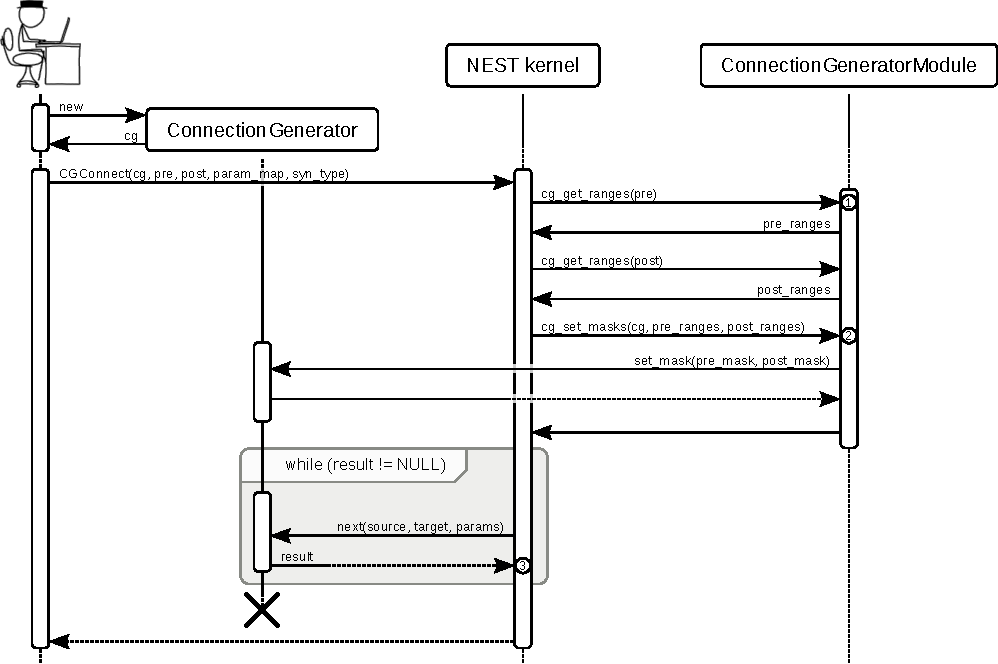
\includegraphics[scale=.8]{figures/sequence_diagram_nest.pdf}
\caption{Sequence diagram of connection generation in NEST using the
  Connection Generator interface. The user first creates a
  ConnectionGenerator object. He then calls PyNEST's function
  \texttt{CGConnect()}. \textcircled{\footnotesize 1} The function
  \texttt{cg\_get\_ranges()} returns all contiguous ranges of gids in
  the given list as vector of closed intervals, still using the gid
  representation. \textcircled{\footnotesize 2} At this point in time,
  the ConnectionGeneratorModule needs to translate NEST gids to CSA
  indices, which run from 0 and enumerate the elements of the given
  pre- and post-synaptic populations. The result of the translation
  (\emph{pre\_mask} and \emph{post\_mask}) is used to set the masks on
  the ConnectionGenerator. \textcircled{\footnotesize 3} The NEST
  kernel iterates the ConnectionGenerator by calling \texttt{next()}
  until there are no more connection. For each connection it receives,
  it creates the connection by calling
  \texttt{Network::connect()}.}\label{fig:sequence_diagram_nest}
\end{figure}

Figure \ref{fig:sequence_diagram_nest} shows the different objects in
NEST that are involved in a user call to \texttt{CGConnect()}. After
setting the masks for the ConnectionGenerator, the NEST kernel
iteratively calls \texttt{next()}, which returns the source index,
target index of the next connection and the parameters of the
connection. The connections are established by calling NEST's basic
\texttt{Network::connect()} function. The extraction of contiguous
ranges and the index translation for the creation of masks is detailed
in Section \ref{sec:creating_masks}.

\subsection{Creating masks}\label{sec:creating_masks}

As explained in Section \ref{sec:csa}, CSA needs to know about which
neurons in the pre- and post-synaptic population are local to the MPI
process, and which are remote. This information is contained in masks,
which are created and set by each NEST process. The masks for CSA are
handed over as a vector of closed intervals that contain the first and
last index of each contiguous range of indices plus an additional skip
value, which is used to describes the ``turn-around'' for a round-robin
distributions of neurons onto MPI processes.

\subsubsection*{Identifying contiguous ranges:}

All elements (neurons or devices) in NEST are identified uniquely by
an integer number, their global id (\emph{gid}). All connection
routines work either on single gids or on lists of gids. When calling
\texttt{CGConnect}, the user supplies two a sorted lists of neurons as
pre- and post-synaptic populations. These lists do not necessarily
have to contain coniguous gids.

The contiguous ranges inside the given lists are found using a binary
search approach, where the left border of a range is always one past
the end of the last range and the right border is searched for. The
following listing contains the procedure to find all contiguos ranges
in a sorted list \emph{n} as a Python script.

First, we initialize \emph{ranges} to an empty list, the left border
(\emph{left}) to 0, and \emph{end} to the last index of \emph{n}.

\begin{pythoncode}
ranges = []
left = 0
end = len(n) - 1
\end{pythoncode}

The following loop will terminate the search when the \emph{end} of
\emph{n} is reached. Until this happens, it always finds the next
right border using \emph{get\_right()} and adds the range between
\emph{left} and \emph{right} to \emph{ranges}. If a new range is
found, left is set to one past the end of the last found range.

\begin{pythoncode}
while True:
    right = get_right(left, (len(n) - left) / 2)
    ranges.append((n[left], n[right]))
    if right == end:
        break
    else:
        left = right + 1
\end{pythoncode}

The task of the \emph{get\_right()} function is to calculate and
return the right border of the contiguous range of gids in \emph{n}
starting at \emph{left}. The element is found using a binary search
with stepsize \emph{step}. First, we check if \emph{left} is already
the index of the last element in \emph{n}. If this is the case, we
return \emph{left} as the right border.

\begin{pythoncode}
def get_right(left, step):
    if left == end:
        return left
\end{pythoncode}

If there are numbers left to be considered, we set \emph{leftmost\_r},
the leftmost right border touched during the search, to \emph{None} to
mark it as unitialized. We then initialize the search index \emph{i}
to the last valid index into \emph{n}, and \emph{last\_i} to \emph{i}.

\begin{pythoncode}
    leftmost_r = None
    i = last_i = end
\end{pythoncode}

In the following loop, we perform the search. If \emph{i} points to
the end of \emph{n} and the distance between \emph{i} and \emph{left}
is the same as between the values \emph{n[i]} and \emph{n[left]}
(i.e. \emph{n[i+1]} equals \emph{n[i]+1} for all \emph{i}), or if
\emph{i} is pointing at the position of the leftmost right border we
found until now (i.e. we're back at an already visited index), we
found the right border of the contiguous range (\emph{last\_i}) and
return it.

\begin{pythoncode}
    while True:
        match = n[i] - n[left] == i - left
        if (i == end and match) or i == leftmost_r:
            return last_i
\end{pythoncode}

We now store the current value of \emph{i} in \emph{last\_i}. This is
the current candidate for the right border.

\begin{pythoncode}
        last_i = i 
\end{pythoncode}

If the range between \emph{n[left]} and \emph{n[i]} is contiguous, we
set \emph{i} to the right by \emph{step} steps, else update the
variable \emph{leftmost\_r} to the current \emph{i} (i.e. the known
leftmost position) and set \emph{i} to the left by \emph{step} steps.

\begin{pythoncode}
        if match:
            i += step
        else:
            leftmost_r = i
            i -= step
\end{pythoncode}

If we reach this point, we have to reduce the search interval
(\emph{step}) to half its size if it is still $>$ 1. This adaptation
is the basis of the binary search.

\begin{pythoncode}
        if step != 1:
            step /= 2
\end{pythoncode}

\subsubsection*{Index translation:}

All elements in NEST are identified by their global id and thus the
range-finding procedure explained in the previous section returns the
ranges in the domain of gids. CSA however, expects neuron indices to
start at 0, i.e. it expects the indices into the pre- and
post-synaptic populations instead of the gids at that positions. This
means that we have to translate indices from NEST to CSA during the
setting of the masks and back when we actually create the connections.

As explained in Section \ref{sec:csa}, the masks for the sources must
contain all local and remote nodes. The \emph{skip} of the mask is
therefore always set to 1. For the sources, the same source mask is
stored \emph{n\_proc} times on each process. The masks for the targets
must only contain the local nodes. This is achieved by i) setting
\emph{skip} to the number of MPI processes upon creation of the mask,
and ii) by taking the index-translated id of the first local neuron as
the first entry of the mask for that range. Together with the skip
this allows to find all local nodes in the range. If this
index-translation renders the resulting range empty (i.e. because the
first local id is beyond the last element of the range), the range is
not added to the mask.

%\subsection{Deserialization}
%On many supercomputers, Python is not available on the compute nodes,
%which would render a purely Python based CSA interface unusable.


%----------------------------------------------------------------------

\section{PyNN connection generators}\label{sec:conn_gen_pynn}
\tbw{To be written}

%----------------------------------------------------------------------

\section{Benchmarks}\label{sec:benchmarks}
\tbw{To be written}

\subsection{CSA vs. Topology vs. RCC}
\tbw{To be written}

%To assess the absolute performance and the scaling behavior of our
%implementation, we conducted several benchmark simulations. All
%simulations consisted of building a random balanced network, which is
%shown in Figure X.
%
%\textbf{Figure 5.}{Block diagram or ingredient table of the benchmark
%  model according to \citet{Nordlie-2009_e1000456}.}\label{fig:05}
%
%\subsubsection{Results}\label{sec:benchmarks_results}
%
%\textbf{Figure 6.}{Scaling plots for different connection methods and
%  networks.}\label{fig:06}

\subsection{simple vs. specialized CSAConnector}
\tbw{To be written}

%----------------------------------------------------------------------

\section{Discussion and outlook}
\tbw{To be written}

%Allow more than 2 parameters to be created by CSA (NEST: make
%number of parameters explicit and check against this value)

%----------------------------------------------------------------------

\section*{Conflict-of-Interest Statement}
The authors declare that the research was conducted in the absence of
any commercial or financial relationships that could be construed as a
potential conflict of interest.

\section*{Acknowledgement}
Partially supported by the Helmholtz Association: HASB and portfolio
theme SMHB, the Jülich Aachen Research Alliance (JARA), the VSR
computation time grant JINB33 on the JUQUEEN supercomputer in Jülich,
and EU Grant 269921 (BrainScaleS). The authors would like to thank
Randall Munroe of http://www.xkcd.org for granting the permission to
use his drawings in the sequence diagrams throughout this article.

%\section*{Supplemental Data}

\bibliographystyle{frontiersinSCNS&ENG}
\bibliography{pns2csa13}

\end{document}
